% !TEX encoding = UTF-8
% !TEX TS-program = pdflatex
% !TEX root = ../tesi.tex

%**************************************************************
\chapter{L'azienda}
\label{cap:azienda}
%**************************************************************

%**************************************************************
\section{Profilo aziendale}
    \textbf{Zextras s.r.l.} nasce a Torri di Quartesolo(VI) nel 2011 come estensione di \textbf{Studio Storti s.r.l.} che opera, dal 1997, nel campo delle soluzioni \gls{opensg}. Sin dall'inizio, l'obiettivo principale di questa società era quello di estendere \gls{zcsg} \textit{Open Source Edition}, uno dei più diffusi strumenti collaborativi per aziende e pubbliche amministrazioni, aggiungendo nuove funzionalità. \\
    Nel corso degli anni è nata e cresciuta \textbf{Zextras Suite}, una raccolta di estensioni che permettono di arricchire \gls{zcsg} con nuove funzionalità utili nel suo utilizzo in ambito professionale.
    Le soluzioni proposte da \textbf{Zextras} con i sui prodotti vengono da subito apprezzate da \textbf{Synacor}, l'azienda che sviluppa e mantiene \gls{zcsg}, la quale decide di includere parte del suo codice nella versione \gls{opensg}. Attualmente i prodotti sviluppati dall'azienda vengono utilizzati da più di 100 milioni di utenti in tutto il mondo.

    \begin{figure}[h]
        \centering
        
\includegraphics[width=0.55\textwidth]{immagini/zextras_logo.png}
        \caption{Logo Zextras}
        \textbf{Fonte:} Zextras
        \label{fig: Logo Zextras}
    \end{figure}

\section{Dominio applicativo}
    \subsection{Zimbra Open Source Edition}
        \textbf{Zextras}, come già accennato, è nata con l'obiettivo di creare nuovi contenuti per \gls{zcsg} facendone quindi il suo \textit{core business}.
        \textbf{Zimbra} è un software collaborativo di gruppo adatto a coordinare e supportare l'attività lavorativa di aziende, pubbliche amministrazioni e altri enti. I principali servizi offerti da questo \textit{software} sono i seguenti:
        \begin{itemize}
            \item posta elettronica;
            \item gestione calendari condivisi e organizzazione eventi;
            \item interfaccia amministratore;
            \item supporto dei servizi su dispositivi mobili.
        \end{itemize}
        Per estendere l'applicativo con ulteriori funzionalità, sviluppate anche da terze parti, è possibile installare un \gls{pluging} che in ambiente \gls{zcsg} viene chiamato \textbf{Zimlet}. \\
        Esistono due versioni di \gls{zcsg}:
        \begin{itemize}
            \setlength\itemsep{0em}
            \item \textbf{Zimbra Open Source Edition}: è la versione su cui lavora \textbf{Zextras} e offre i servizi elecanti in precedenza;
            \item \textbf{Zimbra Network Edition}: è una versione a pagamento che offre alcune funzionalità \gls{closedg} tra cui un protocollo per la sincronizzazione di calendario e contatti e maggiori funzionalità per gli amministratori.
        \end{itemize}
        
        \begin{figure}[h]
            \centering
            
\includegraphics[width=0.55\textwidth]{immagini/zimbra_logo.png}
            \caption{Logo Zimbra}
            \textbf{Fonte:} \href{https://www.zimbra.com/}{zimbra.com}
            \label{fig: Logo Zimbra}
        \end{figure}
        
    \subsection{Zextras Suite}
        \textbf{Zextras Suite} è un'insieme di funzionalità che permettono di aggiungere delle funzionalità a \gls{zcsg} \textit{Open Source Edition} in modo indipendente da quest'ultimo. Ciò permette una configurazione altamente modulare e personalizzabile in base alle necessità dell'utilizzatore. \\
        Questa \textit{suite} offre i seguenti prodotti:
        \begin{itemize}
            \setlength\itemsep{0em}
            \item \textbf{Powerstore}: sistema di ottimizzazione dei dati che permette il risparmio di memoria sui server \textbf{Zimbra};
            \item \textbf{Backup}: motore di \gls{backupg} in \gls{realtimeg};
            \item \textbf{Admin}: strumenti dedicati agli amministratori per la gestione e il monitoraggio dei servizi attivi sull'istanza di \gls{zcsg};
            \item \textbf{Mobile}: gestione e sincronizzazione di posta elettronica, contatti, eventi e calendario su dispositivi mobili tramite protocolli \textit{Exchange} e \textit{EAS 16.0 (ActiveSync)};
            \item \textbf{Chat}: piattaforma di messaggistica istantanea nativamente integrata in \gls{zcsg}, che permette scambio di messaggi e videochiamate;
            \item \textbf{Drive}: piattaforma per la condivisione di file e l'utilizzo di fogli di lavoro condivisi.
        \end{itemize}
\section{Struttura interna}
    L'azienda è suddivisa in diversi settori specializzati, ciò permette di avere un organico fornito di tutte le competenze necessarie per raggiungere gli obiettivi prefissati. Di seguito un elenco che illustra i diversi reparti:
    \begin{itemize}
        \item \textbf{Commercio}: questo reparto, facente parte di \textbf{Studio Storti}, si occupa di gestire tutto ciò che riguarda la parte commerciale e \textit{marketing} dei prodotti proposti dall'azienda;
        \item \textbf{System administration}: questo team svolge l'attività di gestione e manutenzione dell'infrastruttura interna all'azienda che ospita numerosi \textit{server}, i quali erogano i servizi offerti da \gls{zcsg} ai clienti;
        \item \textbf{Team di sviluppo}:
            il team di sviluppo è suddiviso in più aree, ognuna delle quali lavora su un aspetto speficifico dei prodotti di \textbf{Zextras}:
            \begin{itemize}
                \item \textbf{Front-end}: questa divisione progetta e sviluppa tutto ciò che riguarda l'interfaccia grafica delle applicazioni web;
                \item \textbf{Back-end}: questo team si occupa di progettare e implementare l'architettura di tutti i servizi presenti nei prodotti dell'azienda. \'E ulteriormente suddiviso in due team, ciascuno responsabile di un insieme di prodotti diverso;
                \item \textbf{UI/UX Design}: si occupa di progettare l'interfaccia grafica e di studiare l'\gls{userexpg} delle applicazioni web. Lavora a stretto contatto con la divisione front-end;
                \item \textbf{Mobile}: progettazione e sviluppo delle applicazioni per dispositivi mobili.
            \end{itemize}
    \end{itemize}

\section{Processi aziendali}
    I processi sono un tassello di estrema importanza all'interno di un'azienda che si pone degli obiettivi ben definiti, soprattutto quando questi sono particolarmente ambiziosi e raggiungibili tramite lo sviluppo di prodotti complessi e di grandi dimensioni. Sono inoltre fondamentali qual\'{o}ra l'azienda avesse al suo interno dei reparti che svolgono mansioni molto differenti tra loro. \\
    Al fine di orchestrare e mettere in funzione tutti i settori dell'azienda affinché questi lavorino in modo coeso, è necessario ricorrere alla definizione e istanziazione di processi, i quali permettono di stabilire con precisione quali sono le attività da svolgere e il modo più strategico per portarle a termine, al fine di raggiungere gli obiettivi prefissati.
    \subsection{Fornitura}
        La grande diffusione di \gls{zcsg} in molteplici ambiti, contribuisce alla necessità di nuove funzionalità e al miglioramento di quelle già esistenti. Per questo motivo \textbf{Zextras} ottiene spesso nuovi incarichi e nuovi progetti da sviluppare. \\
        La ricerca di nuovi progetti avviene tramite il \textit{CEO} dell'azienda e il \textit{Project Manager}. Oltre all'esigenze dei clienti, nascono dei progetti anche interni dell'azienda stessa che derivano, ad esempio, dalla necessità di migliorare i processi interni con dei nuovi strumenti. \\
        Una volta individuato un possibile progetto, viene fissata una riunione alla quale partecipano i responsabili e il team di sviluppo (formato da gruppi appartenenti a più reparti) che dovrà poi occuparsi del ciclo di vita del nuovo prodotto. Per progetti di grandi dimensioni o particolarmente complessi, la fase di studio di fattibilità dura più tempo e prevede un numero maggiore di riunioni, durante le quali si cerca fin da subito di individuare possibili soluzioni ad alto livello per valutarne la fattibilità. \\
        Dalle riunioni effettuate vengono generati dei verbali, dai quali si estraggono le informazioni più rilevanti che andranno a contribure ai primi contenuti della documentazione. \\
        Quando la soluzione viene approvata da azienda e cliente, si procede con le fasi successive.
    \subsection{Comunicazione}
        Una comunicazione efficiente all'interno del nucleo aziendale è fondamentale per poter essere tutti allineati e coordinati, soprattutto quando è necessario interagire con membri di altri team collocati in altre aree dell'azienda.
        \subsubsection{Strumenti utilizzati}
        \begin{itemize}
            \item \textbf{Posta elettronica}: servizio offerto tramite la posta elettronica di \gls{zcsg};
            \item \textbf{Team}: piattaforma di messaggistica istantanea integrata in \gls{zcsg} sviluppata da \textbf{Zextras};
            \item \textbf{Drive}: piattaforma per la condivisione di documenti su \textit{server} sviluppata dall'azienda;
            \item \textbf{Riunioni}: per discussioni con tutti i membri (o una parte) del team, è possibile indire delle brevi riunioni.
        \end{itemize}

\subsection{Metodologia di sviluppo}
    Per sostenere lo sviluppo di software complessi e dalle dimensioni sostanziose, è necessario avere a disposizione una certa flessibilità ed essere pronti a possibili cambiamenti in termini di requisiti, data anche la tiplogia di servizi che l'azienda sviluppa. Per questo motivo \textbf{Zextras} adotta una filosofia \textit{\gls{agileg}}, preferita rispetto a modelli più rigorosi con l'istanziazione di processi molto forti che portano ad una minore capacità di reagire a cambiamenti imminenti. In particolare, la metodologia di sviluppo adottata in azienda è \textit{Scrum}. In seguito descriverò \textit{Scrum} in relazione a come l'azienda lo attua e da quello che concerne la mia esperienza di stage. \\
    Lo sviluppo di un progetto viene suddiviso in fasi, chiamati \textit{Sprint}, la cui durata può variare da una a quattro settimane. In questo caso, la durata dello \textit{Sprint} era di due settimane.
    Ciascuno \textit{Sprint} ha uno o più obiettivi da portare a termine entro la fine di esso.
    Il \textit{\gls{frameworkg}} \textit{Scrum} prevede lo svolgimento di alcuni eventi e di seguito saranno descritti quelli effettivamente svolti:
    
    \begin{itemize}
        \item \textit{\textbf{Sprint Planning}}: si tratta di una riunione che viene indetta all'inizio di ogni \textit{Sprint}, durante la quale vegono discussi gli obiettivi da raggiungere (\textit{Sprint Goal}). Nello specifico, lo \textit{Scrum Master} ovvero colui che coordina il team sceglie, insieme ai colleghi, i \textit{\gls{taskg}} da svolgere nel corso dello \textit{Sprint} e li inserisce nello \textit{Sprint Backlog}. I \textit{\gls{taskg}} vengono scelti dal \textit{Product Backlog}, ovvero dalla lista completa di funzionalità da implementare nel prodotto. Vengono inoltre stabilite le ore che ciascun membro del team potrà e dovrà dedicare allo sviluppo, alle riunioni e ad altre attività durante il prossimo \textit{Sprint};
        \item \textit{\textbf{Daily Scrum}}: è una riunione della durata di circa 15 minuti che viene svolta ogni inizio giornata con il team di sviluppo (ed eventuali altre persone coinvolte) chiamato anche \textit{Stand-up meeting}. Duranta questa riunione ciascun membro del team parla di ciò che ha svolto il giorno precedente, se ha incontrato ostacoli nello svolgere i suoi \textit{\gls{taskg}} e su quali lavorerà durante la giornata. Per più della metà dello stage, i \textit{daily scrum} del mio team si sono svolti in lingua inglese al fine di migliorare le abilità linguistiche;
        \item \textit{\textbf{Sprint Retrospective}}: questo evento prevede una riunione in cui il team esegue una valutazione retrospettiva sull'andamento dello \textit{Sprint} appena concluso. In particolare vengono analizzate le metriche riguardanti il numero di \textit{\gls{taskg}} portati a termine e gli obiettivi raggiunti. Durante questa riunione viene inoltre svolta un'altra importante attività, ovvero la discussione delle abitudini del team e la ricerca di nuove \textit{best practice}. Per fare ciò, ricorre allo \textit{Starfish Retrospective}, uno schema in cui è possibile individuare i seguenti punti:
            \begin{itemize}
                \item \textit{\textbf{More of}}: elenco delle attività che svolte con più frequenza gioverebbero alla crescrita del team e allo sviluppo del prodotto;
                \item \textit{\textbf{Less of}}: elenco delle attività da ridurre;
                \item \textit{\textbf{Start doing}}: nuove attività individuate di recente che potrebbero migliorare il team e il prodotto;
                \item \textit{\textbf{Keep doing}}: attività che è utile continuare a svolgere;
                \item \textit{\textbf{Stop doing}}: attività il cui svolgimento va interrotto poiché non più necessario oppure perché si tratta di \textit{bad practice}.
            \end{itemize}
            
            \begin{figure}[h]
                \centering
                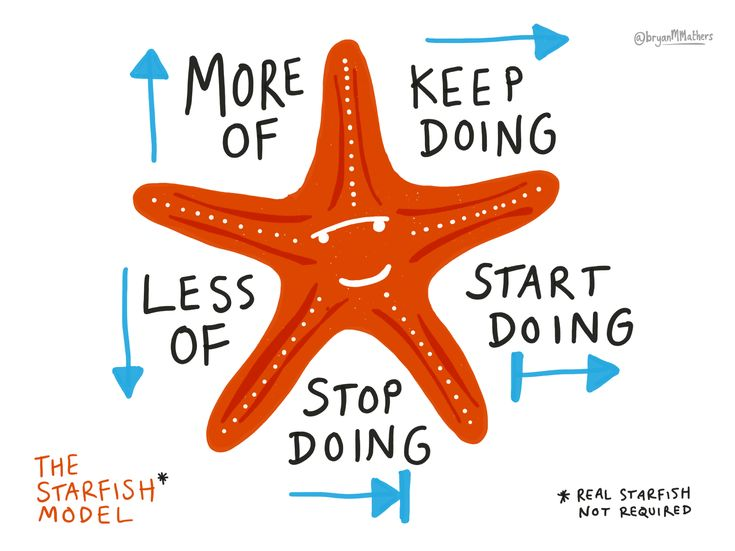
\includegraphics[width=0.7\textwidth]{immagini/starfish.jpg}
                \caption{Starfish retrospective}
                \textbf{Fonte: }\href{https://bryanmmathers.com/the-starfish-model/}{bryanmathers.com}
                \label{fig: Starfish retrospective}
            \end{figure}
            
        \item \textbf{Backlog Refinement}: questa attività, svolta durante lo \textit{Sprint Planning}, consiste nel controllare che tutti gli \textit{item} presenti nel \textit{Product Backlog} siano pronti per essere selezionati e inseriti nello \textit{Sprint Backlog}. Ne vengono rivisti i contenuti, le priorità, le persone assegnate per il loro svolgimento e se necessario, vengono suddivisi in \textit{\gls{taskg}} più piccoli o inclusi in altri già esistenti.
    \end{itemize}

\newpage
    
    \begin{figure}[h]
        \centering
        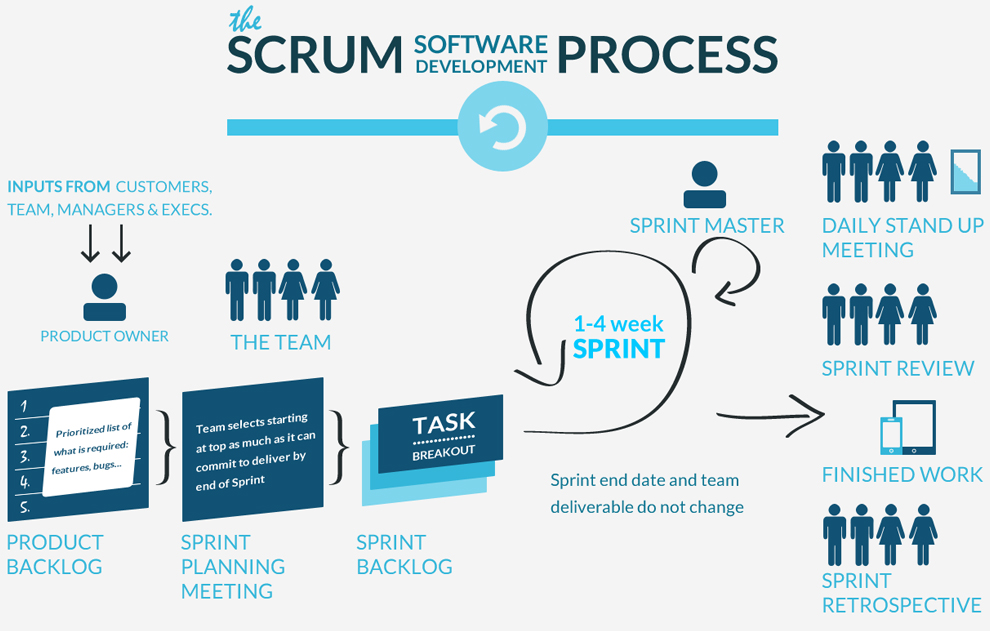
\includegraphics[width=1\textwidth]{immagini/scrum.jpg}
        \caption{Scrum flow}
        \textbf{Fonte:} \href{https://www.ics.ie/news/view/1653}{ICS}
        \label{fig: Scrum flow}
    \end{figure}

\subsection{Gestione di progetto}
    La gestione del progetto viene supportata principalmente da due strumenti:
    \begin{itemize}
        \item \textbf{Atlassian Jira}: è un \textit{\gls{itsg}} molto avanzato che offre la possibilità di gestire tutto ciò che riguarda il \textit{\gls{frameworkg}} \textit{Scrum}, quindi gestione degli \textit{Sprint}, dei \textit{\gls{taskg}} e molto altro. Da \textbf{Jira} è inoltre possibile tracciare le ore impiegate per portare a termine ciascun \textit{\gls{taskg}} fornendo, al termine dello \textit{Sprint}, delle serie storiche con i tempi impiegati dai membri del team e il numero di \textit{\gls{taskg}} portati a termine rispetto a quelli previsti nello \textit{Sprint Backlog}; 
        \item \textbf{\gls{zcsg}}: offre, tra i tanti servizi, il calendario per la gestione degli eventi interni all'azienda, per esempio le riunioni e la possibilità di lavorare su documenti condivisi, per esempio i fogli di calcolo utilizzati per il tracciamento delle ore durante lo \textit{Sprint Planning} come descritto nella sezione precedente. 
    \end{itemize}

\subsection{Documentazione}
    La documentazione di tutti i team di sviluppo è raccolta in un unico punto accessibile a tutti. Per ottenere ciò viene utilizzato il \textit{software} di collaborazione \textbf{Confluence} sviluppato da \textbf{Atlassian}, il quale offre un editor di tipo \textit{\gls{wysiwygg}} che permette di scrivere documenti completi e ben formattati oltre a fornire un sistema di catalogazione molto flessibile e personalizzabile.
    
\newpage

\subsection{Configurazione}
Gli strumenti per il versionamento del codice utilizzati sono i seguenti:
\begin{itemize}
    \item \textbf{Git}: sistema di versionamento;
    \item \textbf{Bitbucket}: servizio che ospita i \textit{\gls{repositoryg}} di tutti i team di sviluppo. Il vantaggio di usare questo strumento è la sua completa integrazione con tutti gli altri strumenti di \textbf{Atlassian} impiegati dall'azienda;
    \item \textbf{GitHub}: servizio che ospita i repository \textit{\gls{opensg}} dell'azienda.
\end{itemize}
Per lo sviluppo di nuove funzionalità viene utilizzato un \textit{\gls{workflowg}} molto simile a \textbf{\textit{Gitflow}}\footnote{\url{https://danielkummer.github.io/git-flow-cheatsheet/}}. Il funzionamento è il seguente:
\begin{enumerate}
    \item Creazione di un nuovo \textit{branch} sul quale sviluppare una nuova funzionalità;
    \item Implementazione nuova funzionalità;
    \item \textit{Pull request} per effettuare il \textit{merge} del codice sul \textit{branch master}, nella quale vengono inseriti alcuni membri del team come revisori, al fine di effettuare una \textit{\gls{codereviewg}} la quale permette di verificare che il codice sia in linea con gli standard di qualità.
    \item Dopo aver messo a punto le correzioni segnalate nella \textit{\gls{codereviewg}} e aver ricevuto l'approvazione dai revisori, avviene il \textit{merge} sul \textit{branch master}.
\end{enumerate}

\subsection{Verifica}
La verifiche che permettono di perseguire la qualità di prodotto avviene tramite \textbf{Jenkins}, un \textit{automation server} che supporta la \textit{\gls{cig}} e la \textit{\gls{cdg}}.
In questo modo è possibile automatizzare il processo di build ad ogni commit sul \textit{\gls{repositoryg}} e rilasciare quest'ultima in ambiente di produzione.
\textbf{Jenkins} permette di aggiungere altre funzionalità al processo di build, per esempio l'analisi statica del codice e la rilevazione di alcune tipologie di \textit{\gls{bugg}}, rendendolo quindi uno strumento molto flessibile e personalizzabile.
Prima della verifica automatizzata vengono effettuate le \textit{\gls{codereviewg}} come descritto nella sezione precedente.
